\ifdefined\included
\else
\documentclass[french, a4paper, 11pt, twoside, pdftex]{StyleThese}
\usepackage{iflang}
\usepackage{bibentry}



%\usepackage[sectionbib]{chapterbib}          % Cross-reference package (Natural BiB)
%\usepackage{natbib}                  % Put References at the end of each chapter
%\usepackage{bibunits}
% Do not put 'sectionbib' option here.
% Sectionbib option in 'natbib' will do.


\usepackage{fancyhdr}                    % Fancy Header and Footer

\usepackage[utf8]{inputenc}
\usepackage[T1]{fontenc}
\usepackage[french]{babel} %
\usepackage{lmodern} \normalfont %to load T1lmr.fd 
\DeclareFontShape{T1}{cmr}{b}{sc} { <-> ssub * cmr/bx/sc }{}
%\hyphenation{gar}

\usepackage{amsmath,amssymb}             % AMS Math
\usepackage{nicefrac}
\usepackage{siunitx}					%% Unites Math SI

\usepackage{blindtext}

\usepackage{datetime}

\usepackage{lipsum} 

\usepackage[inline]{enumitem}

\usepackage{hhline}
%\usepackage[left=1.5in,right=1.3in,top=1.1in,bottom=1.1in]{geometry}
\usepackage[left=1.5in,right=1.3in,top=1.1in,bottom=1.1in,includefoot,includehead,headheight=13.6pt]{geometry}

%%\renewcommand{\baselinestretch}{1.05}

%%%%%%%% Multi-figures avec sub-captions
\usepackage{caption}
\usepackage{subcaption}

% Table of contents for each chapter

\usepackage[nottoc, notlof, notlot]{tocbibind}
\usepackage[nohints]{minitoc}
\setcounter{minitocdepth}{2}
\mtcindent=15pt
% Use \minitoc where to put a table of contents

\usepackage{aecompl}

%% Package cosmetic meilleur layout du texte en jouant sur le spacing par caractères
\usepackage[activate={true,nocompatibility},final,tracking=true,kerning=true,factor=1100,stretch=10,shrink=10]{microtype}
\usepackage[absolute,overlay]{textpos} 
\setlength{\TPHorizModule}{\paperwidth}\setlength{\TPVertModule}{\paperheight}
\sloppy

%%%%%%%%%%% JOLIS TABLEAUX
\usepackage{tabularx}		%\usepackage{tabular}
\usepackage{longtable}
\usepackage{multirow}
\newcommand{\mc}{\multicolumn} 
\newcommand{\mr}[2]{\multirow{#1}{*}{#2}} 	\newcommand{\mrQ}{\multirow{-4}{*}}
\usepackage{booktabs}

\usepackage[usenames,dvipsnames]{xcolor} 

\makeatletter
\newcommand{\ccolor}[3][]{%
	\kern-\fboxsep
	\if\relax\detokenize{#1}\relax
	\expandafter\@firstoftwo
	\else
	\expandafter\@secondoftwo
	\fi
	{\colorbox{#2}}%
	{\colorbox[#1]{#2}}%
	{#3}\kern-\fboxsep
}
\makeatother

%%%%% Insertion graphiques format PGF
\usepackage{pgfplots}
\pgfplotsset{width=\linewidth, compat=1.16}%, compat=1.17}
\usepackage{adjustbox}          %%% PERMET DE LES RECADRER + FACILEMENT


%%%%%%%%%% Bullets de listes sans saut de ligne %%%%%%%%%%
\usepackage{xparse}

\ExplSyntaxOn%
\seq_new:N \l_local_enum_seq

\newcommand{\storethestuff}[1]{%
  \seq_set_from_clist:Nn \l_local_enum_seq {#1}%
}

\newcommand{\dotheenumstuff}{%
\int_zero:N \l_tmpa_int
\seq_map_inline:Nn \l_local_enum_seq {%
    \int_incr:N \l_tmpa_int% Increase the counter
    \item ##1
    % Check whether the list has reached the end -- if so, use '.' instead of ','
    %\int_compare:nNnTF 
    % { \l_tmpa_int } < {\seq_count:N \l_local_enum_seq} 
    % {,} {.}
  }
}
\ExplSyntaxOff

\NewDocumentCommand{\linebullets}{+m}{%
  \storethestuff{#1}%
  \begin{enumerate*}[label={\alph*)},font={\bfseries},itemjoin={{, }}]
    \dotheenumstuff%
  \end{enumerate*}
}

\newcommand{\cmnt}[1]{}  %%%%% AJOUT DE COMMENTAIRE MULTILIGNES


%%%%%%%%%% ECRITURE CARACTERES DANS UN CERCLE %%%%%%%%%%
%\def\circleTxt[#1]{\raisebox{.5pt}{\textcircled{\raisebox{-1pt}{#1}}}}
\newcommand{\ctxt}[1]{\raisebox{.5pt}{\textcircled{\raisebox{-1.2pt}{#1}}}}
% Glossary / list of abbreviations

\usepackage[intoc]{nomencl}
\IfLanguageName{english}{%
\renewcommand{\nomname}{Glossary}
}{ %
\renewcommand{\nomname}{Liste des Abréviations}
}

\makenomenclature

% My pdf code

\usepackage{ifpdf}

\ifpdf
  \usepackage[pdftex]{graphicx}
  \DeclareGraphicsExtensions{.pdf,PDF,.png,PNG,.jpg,JPG}
  \usepackage[pagebackref,hyperindex=true]{hyperref} %% use \autoref{} instead of Table~\ref{}.
  \usepackage{tikz}
  \usetikzlibrary{arrows,shapes,calc}
\else
  \usepackage{graphicx}
  \DeclareGraphicsExtensions{.ps,.eps}
  \usepackage[a4paper,dvipdfm,pagebackref,hyperindex=true]{hyperref}
\fi

\graphicspath{{.}{schemas/}{graphiques/}{tables/}}

%% nicer backref links. NOTE: The flag ThesisInEnglish is used to define the
% language in the back references. Read more about it in These.tex

\IfLanguageName{english}{
\renewcommand*{\backref}[1]{}
\renewcommand*{\backrefalt}[4]{%
\ifcase #1 %
(Not cited.)%
\or
(Cited in page~#2.)%
\else
(Cited in pages~#2.)%
\fi}
\renewcommand*{\backrefsep}{, }
\renewcommand*{\backreftwosep}{ and~}
\renewcommand*{\backreflastsep}{ and~}
}{
\renewcommand*{\backref}[1]{}
\renewcommand*{\backrefalt}[4]{%
\ifcase #1 %
(Non cité.)%
\or
(Cité en page~#2.)%
\else
(Cité en pages~#2.)%
\fi}
\renewcommand*{\backrefsep}{, }
\renewcommand*{\backreftwosep}{ et~}
\renewcommand*{\backreflastsep}{ et~}
}

% Links in pdf
\usepackage{color}
\definecolor{linkcol}{rgb}{0,0,0.4} 
\definecolor{citecol}{rgb}{0.5,0,0} 
\definecolor{linkcol}{rgb}{0,0,0} 
\definecolor{citecol}{rgb}{0,0,0}
% Change this to change the informations included in the pdf file

\hypersetup
{
bookmarksopen=true,
pdftitle="Prévention des fautes temporelles sur architectures multicœur pour les systèmes à criticité mixte",
pdfauthor="Daniel LOCHE", %auteur du document
pdfsubject="Thèse", %sujet du document
%pdftoolbar=false, %barre d'outils non visible
pdfmenubar=true, %barre de menu visible
pdfhighlight=/O, %effet d'un clic sur un lien hypertexte
colorlinks=true, %couleurs sur les liens hypertextes
pdfpagemode=UseNone, %aucun mode de page
%pdfpagelayout=DoublePage, %ouverture en simple page
pdffitwindow=true, %pages ouvertes entierement dans toute la fenetre
linkcolor=linkcol, %couleur des liens hypertextes internes
citecolor=citecol, %couleur des liens pour les citations
urlcolor=linkcol %couleur des liens pour les url
}

% definitions.
% -------------------

\setcounter{secnumdepth}{3}
\setcounter{tocdepth}{2}

% Some useful commands and shortcut for maths:  partial derivative and stuff

\newcommand{\pd}[2]{\frac{\partial #1}{\partial #2}}
\def\abs{\operatorname{abs}}
\def\argmax{\operatornamewithlimits{arg\,max}}
\def\argmin{\operatornamewithlimits{arg\,min}}
\def\diag{\operatorname{Diag}}
\newcommand{\eqRef}[1]{(\ref{#1})}
\newcommand{\nline}{\smallbreak\noindent}

\usepackage{rotating}                    % Sideways of figures & tables

% \usepackage{txfonts}                     % Public Times New Roman text & math font
  
%%% Fancy Header %%%%%%%%%%%%%%%%%%%%%%%%%%%%%%%%%%%%%%%%%%%%%%%%%%%%%%%%%%%%%%%%%%
% Fancy Header Style Options

\pagestyle{fancy}                       % Sets fancy header and footer
\fancyfoot{}                            % Delete current footer settings

%\renewcommand{\chaptermark}[1]{         % Lower Case Chapter marker style
%  \markboth{\chaptername\ \thechapter.\ #1}}{}} %

%\renewcommand{\sectionmark}[1]{         % Lower case Section marker style
%  \markright{\thesection.\ #1}}         %

\fancyhead[LE,RO]{\bfseries\thepage}    % Page number (boldface) in left on even
% pages and right on odd pages
\fancyhead[RE]{\bfseries\nouppercase{\leftmark}}      % Chapter in the right on even pages
\fancyhead[LO]{\bfseries\nouppercase{\rightmark}}     % Section in the left on odd pages

\let\headruleORIG\headrule
\renewcommand{\headrule}{\color{black} \headruleORIG}
\renewcommand{\headrulewidth}{1.0pt}
\usepackage{colortbl}
\arrayrulecolor{black}

\fancypagestyle{plain}{
  \fancyhead{}
  \fancyfoot{}
  \renewcommand{\headrulewidth}{0pt} %%%%%%%%%%%%%%%%%%%%%%%%%%%%%%%%%%%%%%%%%%%%%%%%%%%%%%%%%%%%%%%%%%%%%%%%%%%%%%%%%%%%%
}

%\usepackage{MyAlgorithm}
%\usepackage[noend]{MyAlgorithmic}
%\usepackage[ED=EDSYS-SystEmb, Ets=INP]{tlsflyleaf}

%%% Clear Header %%%%%%%%%%%%%%%%%%%%%%%%%%%%%%%%%%%%%%%%%%%%%%%%%%%%%%%%%%%%%%%%%%
% Clear Header Style on the Last Empty Odd pages
\makeatletter

\def\cleardoublepage{\clearpage\if@twoside \ifodd\c@page\else%
  \hbox{}%
  \thispagestyle{empty}%              % Empty header styles
  \newpage%
  \if@twocolumn\hbox{}\newpage\fi\fi\fi}

\makeatother
 
%%%%%%%%%%%%%%%%%%%%%%%%%%%%%%%%%%%%%%%%%%%%%%%%%%%%%%%%%%%%%%%%%%%%%%%%%%%%%%% 
% Prints your review date and 'Draft Version' (From Josullvn, CS, CMU)
\newcommand{\reviewtimetoday}[2]{\special{!userdict begin
    /bop-hook{gsave 20 710 translate 45 rotate 0.8 setgray
      /Times-Roman findfont 12 scalefont setfont 0 0   moveto (#1) show
      0 -12 moveto (#2) show grestore}def end}}
% You can turn on or off this option.
% \reviewtimetoday{\today}{Draft Version}
%%%%%%%%%%%%%%%%%%%%%%%%%%%%%%%%%%%%%%%%%%%%%%%%%%%%%%%%%%%%%%%%%%%%%%%%%%%%%%% 

\newenvironment{maxime}[1]
{
	\def\Arg{#1}
\vspace*{0cm}
\hfill
\begin{minipage}{0.6\textwidth}%
%\rule[0.5ex]{\textwidth}{0.1mm}\\%
\hrulefill $\:$ \\%$\:$ {\bf #1}\\
%\vspace*{-0.25cm}
\it 
}%
{%
	
\hrulefill $\:$ {\bf \Arg}
\vspace*{0.5cm}%
\end{minipage}
}

\let\minitocORIG\minitoc
\renewcommand{\minitoc}{\minitocORIG \vspace{1.5em}}

%\usepackage{slashbox}

\newenvironment{bulletList}%
{ \begin{list}%
	{$\bullet$}%
	{\setlength{\labelwidth}{25pt}%
	 \setlength{\leftmargin}{30pt}%
	 \setlength{\itemsep}{\parsep}}}%
{ \end{list} }


%%%%%%% Outils pour \comment \alert \add %%%%%
\usepackage{easyReview}
\usepackage{soulutf8} % for accented letters

\let\newalert\alert
\renewcommand{\alert}[1]{\textit{\newalert{#1}}}

%\usepackage[commandnameprefix=ifneeded]{changes} %% \chhighlight and \chcomment to avoid collision with easyReview
\renewcommand{\epsilon}{\varepsilon}

% centered page environment

\newenvironment{vcenterpage}
{\newpage\vspace*{\fill}\thispagestyle{empty}\renewcommand{\headrulewidth}{0pt}}
{\vspace*{\fill}}

\usepackage{tablefootnote}

%%%%%% MISE EN FORME CADRES DEFINITIONS/THEOREMES/LEMES %%%%%%%%%%
\usepackage{amsthm}  % for theoremstyle

\theoremstyle{plain} 
\newtheorem{theorem}{Théorème}[section]
\newtheorem{corollary}{Corolaire}[theorem]

%\theoremstyle{lemma}
%\newtheorem{lemma}[theorem]{Lemme}


\theoremstyle{definition}
\newtheorem{definition}[theorem]{Définition}


\cmnt{
	\usepackage{ntheorem} %\usepackage{amsthm}  % for theoremstyle
	%\usepackage{mdframed}
	\usepackage[most]{tcolorbox}
	
	\theoremstyle{plain} 
	\theoremindent20pt
	\theoremheaderfont{\normalfont\bfseries\hspace{-\theoremindent}}
	\newtheorem{theorem}{Théorème}[section]
	\newtheorem{corollary}{Corolaire}[theorem]
	
	\theoremstyle{plain}
	\newtheorem{lemma}[theorem]{Lemme}
	
	
	\tcolorboxenvironment{theorem}{
		blanker,
		breakable,
		before skip=\topsep,
		after skip=\topsep,
		borderline west={1pt}{10pt}{double, shorten <=12pt}
	}
	
	\theorembodyfont{\normalfont}
	\theoremindent20pt
	\theoremheaderfont{\normalfont\bfseries\hspace{-\theoremindent}}
	\newtheorem{definition}[theorem]{Définition}
	
	
	\tcolorboxenvironment{definition}{
		blanker,
		breakable,
		before skip=\topsep,
		after skip=\topsep,
		borderline west={1pt}{10pt}{shorten <=12pt}
	}
}

\cmnt{ 
	\begin{theorem}
		Ceci est un Théorème.
	\end{theorem} 
	
	\begin{corollary}
		Ceci est un Corollaire.
	\end{corollary}
	
	\begin{definition}
		Ceci est une Définition.
	\end{definition}
	
	\begin{lemma}
		Ceci est un Lemme.
	\end{lemma}
}

\def\UrlBigBreaks{\do\/\do-\do:}
\usepackage{url}

\sloppy
\begin{document}
\setcounter{chapter}{5} %% Numéro du chapitre précédent ;)
\dominitoc
\faketableofcontents
\fi

\chapter{Cas d'implémentation de l'Agent de Monit. \& Contrôle}
\minitoc

%%%% CONTENU %%%%
    \section{Framework et Architecture Logicielle}
    
        \subsection{Plateforme Matérielle}
                        The platform used for the experimentation is a barebone computer equipped with a processor Intel Core i5-8250U. This processor embeds 4 cores. It has 3 caches level, L1, L2 and L3 (shared), with respectively 32 KiB/core, 256 KiB/core and 8 Mib (shared). We fixed its frequency to 1400MHz and disabled hyper-threading for our tests.
        \subsection{Support Logiciel}
                    We used Linux (Linux Mint xfce 18.04 distribution) to mix general purpose and real-time applications with different scheduling policies (\cite{wong_towards_2008}, \cite{lelli_efficient_2011}). Its versatility grants easier compatibility with benchmarking suites. Moreover, by adding Xenomai (v. 3.1) real-time co-kernel~\cite{gerum_xenomai_2004}, it is possible to get closer to real-time applications with latencies lowered from milliseconds down to microseconds. It also grants an API for real-time application development, used for the MCA framework.
                        
                        Notably, POSIX enables to force tasks execution to dedicated cores and change both priority and scheduling policy. As we are in a controlled context that suppose no malicious behavior, we do not implement mechanisms like memory protection or strong space isolation policies. As stated before, vanilla Linux Kernel is not made for hard real-time application. That is mainly because kernel is not preemptive on most parts of it, this can cause high latency for real-time interrupts, from kernel code execution that could be linked to non-critical applications. % due to its non-preemptiveness. It causes high latencies to the system due to kernel and drivers interrupts.
                        Therefore, we add a Xenomai co-kernel to improve latency down to micro-seconds and run our MCA to respect desired real-time constraints.
                        Please note that from Linux point of view, ``threads" and ``processes" are equivalent and correspond to ``tasks" for us.
            
                        Threads are assigned 2 parameters, a scheduling policy and a static priority (\textit{sched\_priority}). Both are considered by the global scheduler. It first gathers the threads by priority level to execute highest priority processes first. Then for a same priority level, the scheduling policy of each task will define which one to run first. For normal processes the priority level is ignored (considered at 0) to be executed following the CFS policy. This way, a real-time process with a priority level from 1 (lowest) to 99 (highest), always run before them. The threads' scheduling policy defines how they are inserted into the list of same priority level and how they move in this list, all processes being preemptive.  We can list 3 real-time policies for real-time process: FIFO, EDF and Round-Robin. \\
                        For this purpose, Linux allows to bound threads to cores. For a processor with $j$ cores, every thread has a core affinity represented by an array of $j$ Booleans. Each of these Booleans of affinity $b_{Ti}$ indicates if the thread $T$ can be executed on the core $i$. By default, every normal process has a core affinity of $\begin{pmatrix}1 & 1 & 1 & 1\end{pmatrix}$, for a quad-core processor, meaning that it can be executed by every core. It makes it easier for the scheduler to balance load between every core. But for our case and when it comes to run hard real-time applications, it is interesting to use such affinity. This way, it will be possible to isolate our MCA on an isolated core and bound the benchmark processes to the other threads.
                        Xenomai is a real-time kernel that can be installed as a co-kernel to a classic Linux distribution as presented in deep by \cite{gerum_xenomai_2004}. Our framework and experiments are implemented on the real-time APIs proposed by Xenomai 3.1.
            %in order to implement it and add measurements instrumentation. %Xenomai version installed is 3.0.5, from tutorial \cite{hoarau_beta_2017}.
                        In such configuration, it adds an interruption pipeline (ADEOS) directly between the hardware and OS low-level software (i.e. Hardware Abstraction Layer, OS Kernel and drivers). This enables to catch all the interrupts and distribute them in priority to Xenomai real-time kernel.
                        Threads executed with Xenomai are executed either in primary or secondary mode. In both cases they are memory-protected from other processes. By default, Xenomai threads starts in primary mode. They get directly access to Xenomai API and are scheduled by its real-time scheduler. A Xenomai thread can however use kernel API with system calls. When it happens, the Xenomai tasks goes temporarily to the Linux scheduler and automatically goes back to Xenomai domain once done. As the priority system used on primary mode is compatible with the secondary one, the Xenomai tasks keep their highest priority status. It makes the mode switch transparent.
            
                        All things considered, we mainly use Xenomai to get a significant latency gain (divided by up to 10) for the critical tasks. We can stay on the classic Linux domain for our non-critical tasks.
            
                    Such OS configuration allows us to specify a per-task core allocation and priority level. Linux scheduler as explained in~\cite{ishkov_complete_2015} selects tasks first by priority level, (from 1 to 99 for real-time tasks domain). Then for a given priority level, multiple scheduling policies are possible: Global Earliest Deadline First, FIFO, Round-Robin, and other best-effort policies. To test a system using classic Round-Robin for instance, every task are launched at same priority level with Round-Robin policy. We use Rate-Monotonic scheduling policy for our tests this way.
                        
    \section{Benchmark MiBench}
        \subsection{Présentation}
        MiBench~\cite{guthaus_mibench_2001} plays the role of the task set to constitute our experimental workload. This benchmark suite gives source code for 30+ standalone binaries classified in six domains~: automotive, security, network, telecommunication, office and consumer. Those tasks do different jobs similar to ones in these domains, with different levels of complexity that is of high interest for us.

            To run an artificial system load as a ``worst-case" cache, memory, CPU use and I/O stress, we use Linux \textit{Stress-ng} tool presented in~\cite{king_stress-ng_2019}. 


            As we do not have yet real industrial application for testing, for now the MiBench Benchmark suite~\cite{guthaus_mibench_2001} has been used for our experiments. The objective is to use applications similar as much as possible to computation profiles that could be found in real applications, in order to reproduce memory containment and resource usage close to real cases. 
            %We lack real applications to test, but 
            
            MiBench consists of a large panel of tasks with different memory needs and execution profiles to mimic existing applications. We have at disposal applications from 5 different domains, as presented in the \autoref{MiBenchTable}. It is used here to validate the framework and put into practice our experiments.\\
            \begin{table}[!t]
                %% increase table row spacing, adjust to taste
                \renewcommand{\arraystretch}{1.3}
                % if using array.sty, it might be a good idea to tweak the value of
                %\extrarowheight as needed to properly center the text within the cells
                \caption{MiBench selected tasks}
                \label{MiBenchTable}
                \centering
                %% Some packages, such as MDW tools, offer better commands for making tables
                %% than the plain LaTeX2e tabular which is used here.
                \begin{tabular}{|c||c|}
                    \hline
                    Automotive  & basicmath, bitcount, qsort, susan (smooth/edges/corners)\\
                    \hline
                    Network     & dijkstra, patricia                                        \\
                    \hline
                    Consumer    & jpeg (code \& decode), typeset                            \\
                    \hline
                    Office      & stringsearch                                              \\
                    \hline
                    Security    & blowfish, rijndael, sha                                   \\
                    \hline
                    Telecom     & adpcm (coding \& decoding), CRC32, FFT, gsm               \\
                    \hline
                \end{tabular}
            \end{table}
            We selected a set of 16 applications from MiBench for our experiments. Most of them exists in ``small" and ``large" version that allows to change proportionally their execution time and resource needs. Also, some of these tasks may have several variants according to setup parameters. For instance, $Sunsan$ has 6 different variants: edge detection, corner detection and smoothing, all 3 existing in both ``small" and ``large" version which works with a bigger image for processing. This way, those 16 applications leads to 45 different possible tasks for our experiments. It enables to test different combination following the ``size" and number of tasks but also the kind of tasks we use.
            Tasks profile classification were already made by Guthaus \& al. in~\cite{guthaus_mibench_2001} and detailed work about their memory consumption can be found in~\cite{blin_understanding_2016}. 
        
        \subsection{Demandes d'adaptation/modification des tâches}
    \section{Agent de Monitoring et Control}
            \begin{figure}
                \centering
                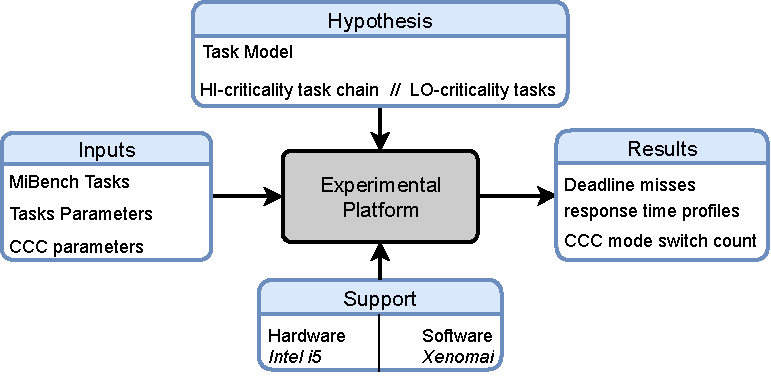
\includegraphics[width=\linewidth]{ExperimentsArch}
                \caption{Experimental Platform structure\label{fig:expe}}
            \end{figure}
    
%\chapter{Bilan de l'expérimentation}
    \section{Solutions adoptées à la complexité d'implémentation}
        Difficultés rencontrées dans la mise en place de ce concept et leçons apprises (en cas de volonté de reproduction)


\ifdefined\included
\else
\bibliographystyle{StyleThese}
\bibliography{these}
\end{document}
\fi